
\documentclass[ucs]{beamer}

\usetheme{GSyC}
%\usebackgroundtemplate{\includegraphics[width=\paperwidth]{gsyc-bg.png}}


\usepackage[spanish]{babel}
\usepackage[utf8x]{inputenc}
\usepackage{graphicx}
\usepackage{amssymb} % Simbolos matematicos


% Metadatos del PDF, por defecto en blanco, pdftitle no parece funcionar
   \hypersetup{%
     pdftitle={Virtualización I},%
     %pdfsubject={Diseño y Administración de Sistemas y Redes},%
     pdfauthor={GSyC},%
     pdfkeywords={},%
   }
%


% Para colocar un logo en la esquina inferior de todas las transpas
%   \pgfdeclareimage[height=0.5cm]{gsyc-logo}{gsyc}
%   \logo{\pgfuseimage{gsyc-logo}}


% Para colocar antes de cada sección una página de recuerdo de índice
%\AtBeginSection[]{
%  \begin{frame}<beamer>{Contenidos}
%    \tableofcontents[currentframetitle]
%  \end{frame}
%}


%\newboolean{detallado}
%\setboolean{detallado}{false}
%\newcommand{\opcional}[1]{\ifthenelse{\boolean{detallado}}{#1}{}}


\definecolor{darkred}{rgb}  {1.0, 0.0, 0.0}
\definecolor{darkgreen}{rgb}{0.0, 0.4, 0.0}
\definecolor{darkblue}{rgb} {0.0, 0.0, 0.8}

% for resalted text
\newcommand{\res}[1]{\textcolor{darkred}{#1}}
% for different text
\newcommand{\dif}{\textsl}
% for reserved words
\newcommand{\rw}[1]{\textrm{\textbf{#1}}}
% for commands
\newcommand{\com}[1]{\textrm{\textbf{#1}}}






\begin{document}

% Entre corchetes como argumento opcional un título o autor abreviado
% para los pies de transpa
\title[Virtualización I]{Virtualización I}
%\subtitle{Diseño y Administración de Sistemas y Redes}
\author[GSyC]{Escuela Técnica Superior de Ingeniería de Telecomunicación\\
Universidad Rey Juan Carlos}
\institute{gsyc-profes (arroba) gsyc.urjc.es}
\date[2017]{Septiembre de 2017}



%% TÍTULO
\begin{frame}
  \titlepage
  % Oportunidad para poner otro logo si se usó la opción nologo
  % \includegraphics[width=2cm]{logoesp}  
\end{frame}



%% LICENCIA DE REDISTRIBUCIÓN DE LAS TRANSPAS
%% Nota: la opción b al frame le dice que justifique el texto
%% abajo (por defecto c: centrado)
\begin{frame}[b]
\begin{flushright}
{\tiny
\copyright \insertshortdate~\insertshortauthor \\
  Algunos derechos reservados. \\
  Este trabajo se distribuye bajo la licencia \\
  Creative Commons Attribution Share-Alike 4.0\\
}
\end{flushright}  
\end{frame}



%% ÍNDICE
\begin{frame}
  \frametitle{Contenidos}

%\begin{tiny}
  \tableofcontents
%\end{tiny}

\end{frame}





\section{Máquinas Virtuales}
%%---------------------------------------------------------------
\begin{frame}[fragile]
\frametitle{Máquinas Virtuales}

Máquina Virtual: Software que crea una capa de abstracción, 
ofreciendo una máquina diferente a la máquina original
% hasta un pentium es una máquina virtual, muchas
% instrucciones son realmente funciones

Las máquinas virtuales que nos interesan en administración de 
sistemas suelen ofrecer a un sistema operativo la percepción
de una máquina física
% pero pj la mv java tiene por encima una aplicación, y por
% debajo una máquina que no existe físicamente (en tiempos
% sun pretendía eso, seguramente para vender hw ahora que
% sparc no vende gran cosa. El problema es que el hw java
% nativo es mucho menos eficiente que uno de propósito general.
% Pasó lo mismo cuando intentaron hacer procesadores prolog,
% (lenguaje lógico, ni funcional ni imperativo)
% que para cuando lo desarrollaron, un procesador convencional
% con un intreprete convencional iba mucho mejor)


\begin{itemize}	
\item
Las aplicaciones y los usuarios dentro de la máquina virtual se relacionan
con la capa de abstracción y no con la plataforma real

\item 
La máquina virtual puede implementar diversos dispositivos virtuales (disco, dispositivos
de red, etc) diferentes a los de la plataforma real

\end{itemize}


\end{frame}



%%---------------------------------------------------------------
\begin{frame}[fragile]
\begin{itemize}
\item
La tecnología sobre Máquinas Virtuales está muy madura. La terminología, no. 
Es frecuente encontrarse 
con el distintos nombres para el mismo concepto, o incluso el mismo nombre para cosas distintas
\item
\emph{Guest}: Sistema Operativo de la máquina virtual

\emph{Host}: Sistema Operativo de la máquina real
\end{itemize}

\end{frame}



%%---------------------------------------------------------------
\begin{frame}[fragile]

\begin{minipage}{5cm}
\begin{figure}
\centerline{\includegraphics[width=6.9cm]{figs/cajas_hiperv}}
\end{figure}
\end{minipage} \hfill
\
\begin{minipage}{4cm}
\begin{itemize} 
\item
La máquina virtual se comporta como una aplicación más en el \emph{host} 
\item
El \emph{guest} percibe la máquina virtual como si fuera hardware real
%\item 
\end{itemize}
\end{minipage}\hfill

\begin{footnotesize}
Uno de los modelos posibles: máquina virtual de sistema
\end{footnotesize}
\end{frame}



%%---------------------------------------------------------------
\subsection{Utilidad de las máquinas virtuales}
%%---------------------------------------------------------------
\begin{frame}[fragile]
\frametitle{Utilidad de las máquinas virtuales}
Tecnología tradicional y actual, con muchas utilidades
\begin{itemize}	
\item
Ejecutar aplicaciones hechas para una plataforma sobre una plataforma diferente: 
p.e Microsoft Windows sobre Mac OS, Java Virtual Machine
 
\item
Ofrecer un entorno seguro donde experimentar (\emph{sandbox})
\begin{itemize}	
\item
Docencia
\item
Probar aplicaciones en desarrollo
\item
Probar aplicaciones o webs no confiables
\end{itemize}
\item
Señuelos (\emph{Honeypots})
\item
Empresas de \emph{hosting} pueden ofrecer servidores virtuales (alimentación y conectividad
redundante, soporte 24/365, etc)


\end{itemize}
\end{frame}

%--------------------------------------------------------------------

\begin{frame}[fragile]
\begin{itemize}

\item
Respaldo (\emph{backup}) de máquinas enteras, no solo de datos. Ante un pequeño
problema o un gran desastre, la máquina virtual se recupera inmediatamente
\item
Seguridad: Cortafuegos, perímetros de seguridad,...
\item
Portabilidad: Moviendo un directorio se puede mover la máquina virtual
de una máquina real a otra
%Puedes ofrecer a tus usuarios una máquina virtual en un pendrive
%en vez de un portátil
\item
Independencia del Hardware, p.e. homogeneizar un conjunto de máquinas diferentes
\item
...
\end{itemize}
\end{frame}



%%---------------------------------------------------------------
\subsection{Inconvenientes de las máquinas virtuales}
%%---------------------------------------------------------------
\begin{frame}[fragile]
\frametitle{Inconvenientes de las máquinas virtuales}

Inconveniente principal: pérdida de rendimiento

Aunque no siempre
\begin{itemize}	
\item
La máquina \emph{real} tal vez no existe (p.e. java)
\item
Existe, pero es una máquina de propósito específico.

Un guest sobre un host de propósito general puede ser
más eficiente
\end{itemize}

\end{frame}





%%---------------------------------------------------------------
\section{Tipos de Máquina Virtual}
%%---------------------------------------------------------------


%%---------------------------------------------------------------
%\begin{frame}[fragile]
%\frametitle{Tipos de Máquina Virtual}
%\begin{itemize}
%\item
%Emulación Completa, también llamada Virtualización Completa
%\item
%Virtualización
%\item
%Máquinas Virtuales Cooperativas
%\item
%Paravirtualización
%\item
%Virtualización Nativa
%\end{itemize}
%
%Parte de la funcionalidad de las máquinas virtuales puede
%obtenerse con técnicas alternativas
%
%\end{frame}


\subsection{MV de proceso y de sistema}
%%---------------------------------------------------------------
\begin{frame}[fragile]
\frametitle{MV de proceso y de sistema}

Según su grado de equivalencia sobre una máquina hardware, las máquinas virtuales
se pueden clasificar en 
\begin{itemize}
\item
Máquinas virtuales de sistema

Proporcionan un entorno completo y persistente para ejecutar un sistema operativo y sus procesos

Ej: VirtualBox, Xen

\item
Máquinas virtuales de proceso

Proporcionan una plataforma para ejecutar un único proceso


\begin{itemize}
\item
Contenedores
\item
Máquina virtual de java, .NET

Este tipo no lo consideramos dentro del ámbito
de la administración de sistemas y no lo tratamos aquí
\end{itemize}




\end{itemize}

\end{frame}



%%---------------------------------------------------------------
\subsection{Emulación Completa o Virtualización Completa}
%%---------------------------------------------------------------

\begin{frame}[fragile]

\frametitle{Emulación Completa o Virtualización Completa}
\emph{Whole-system virtualization}.
\begin{footnotesize}
%Estos términos no siempre se usan de la misma forma
\end{footnotesize}
%\footnote{Estos términos no siempre se usan de la misma forma}
%Son técnicas similares. 
Se emula memoria, disco y otros dispositivos, también la CPU:
%\begin{itemize}
%\item
%Instrucción a instrucción en la emulación
%\item
%Por bloques en la virtualización
%\end{itemize}

Al emular la CPU, son especialmente lentos. La arquitectura Intel 
tradicional ofrecía muy pocas facilidades
% Los desarrolladores de sistemas (Microsoft) suelen pedir
% a los desarrolladores de cpus (intel) instrucciones de alto
% nivel que hagan cosas, a lo que estos suelen resistirse.
% Pero en ocasiones han aceptado: pj intrucciones sobre chorros de bytes para 
% procesar multimedia. Instrucciones para MV

Permiten que \emph{guest} y \emph{host} trabajen con diferente
ISA (\emph{instruction set architecture})

\end{frame}

%--------------------------------------------------------------------

\begin{frame}[fragile]
%\begin{itemize}

Ejemplos: QEMU, Bochs. 
\begin{itemize}
\item
Emulan una CPU intel, incluso cuando se ejecutan
sobre intel. 
\item
Ambos son libres, disponibles para diversos \emph{hosts}.
\item
Pueden ejecutar distintos
\emph{guest}, pero siempre para intel
\end{itemize}



\end{frame}

\subsection{Virtualización}
%%----------------------------------------------
\begin{frame}[fragile]

\frametitle{Virtualización}
\begin{itemize}
\item
Al virtualizador también se le llama \emph{hipervisor}
%\item
%Además de virtualizador, se usa el término
%\emph{hypervisor} y \emph{Virtual Machine Monitor}
% al SO se la llamaba supervisor, supervisando al supervisor
% estaba el hypervisor. Con un hypervisor no es que te curres
% una emulación de una soundblaster, sino que el hypervisor
% puede llamar al driver soundblaster de otro SO

\item
Se emula memoria virtual, disco y dispositivos

Ejemplo: VMware emula tarjeta de audio SoundBlaster 16 y
tarjeta ethernet
AMD PCnet II. Cualquier aplicación en el \emph{guest}
percibe este hardware


\item
No se emula la CPU.
Por tanto 
\emph{guest} y \emph{host} 
tienen que usar la misma arquitectura
\end{itemize}


\end{frame}



%%---------------------------------------------------------------
\begin{frame}[fragile]

\res{VMware}. Virtualizador. Software muy maduro. Versiones comerciales y versiones \emph{freeware} 
(con los años va aumentando el número de versiones freeware)
\begin{itemize}
\item
VMware Workstation, workstation player. Para host Windows y Linux. Permite crear y ejecutar máquinas virtuales 
\item
VMware Fusion. Similar a VMWare Workstation, para Mac OS
\item
VMware ESXi. Verdarero Sistema Operativo. Se ejecuta directamente sobre el hardware
\item
VMware vSphere. Computación en la nube. Basado en ESXi
\end{itemize}


\end{frame}




%%---------------------------------------------------------------
\begin{frame}[fragile]

%\res{Windows Virtual PC}
%% desarrollado por Connectix y comprado por Microsoft
%\begin{itemize}	
%\item
%Software propietario de Microsoft, algunas versiones son \emph{freeware}
%\item
%El \emph{guest} puede ser prácticamente cualquier SO para intel
%\item
%Dos versiones
%\begin{enumerate}
%\item  
%Para \emph{hosts} Microsoft Windows. Es un virtualizador
%\item  
%Para \emph{hosts} Mac OS. Es un virtualizador completo. Los Mac OS basados
%en PowerPC (anteriores a 2006) solo tenían esta opción para ejecutar Windows
%
%\end{enumerate}
%
%
%\end{itemize}


\res{Parallels Desktop}

\begin{itemize}	
\item
Virtualizador para los Mac OS basados en Intel
\item 
\emph{guest} soportados: Microsoft Windows, Linux, FreBSD, Sun Solaris y algunos otros
\end{itemize}

(los Mac posteriores a 2006, basados en Intel, pueden ejecutar Windows en nativo con Boot Camp)


%kqemu . versión de qemu que incluye virtualización. Recientemente
%liberado como gpl

\end{frame}



%%---------------------------------------------------------------
\begin{frame}[fragile]
\res{VirtualBox}
\begin{itemize}
\item
Virtualizador, muy similar a VMware
\item
Desarrollado por Innotek. Sun compra Innotek en 2008. Oracle compra Sun en 2009

\begin{itemize}
\item
Virtual Box Open Source Edition
\item
VirtualBox. Software Comercial. Gratuito para uso personal y académico

Incluye alguna característica adicional, como soporte USB. sATA, iSCSI, Remote Display Protocol (RDP) Server
\end{itemize}

\end{itemize}

\end{frame}



%--------------------------------------------------------------------
\subsection{Paravirtualización}
%--------------------------------------------------------------------

\begin{frame}[fragile]
\frametitle{Paravirtualización}


Similar a la virtualización, pero
exige un versión ligeramente modificada del \emph{guest}

El rendimiento es normalmente mayor que el de los tipos anteriores

Xen

\begin{itemize}	
\item
Muy extendido
\item
Hay una versión libre que permite Linux sobre Linux
\item
Hay versiones comerciales que permiten Windows sobre Windows
\item
Los drivers están paravirtualizados, son más eficientes.
(En un virtualizador, los drivers son drivers hw normales)
\item
También hay que modificar el \emph{guest} (Xen lo llama \emph{Dom0})

\end{itemize}	

\end{frame}

%--------------------------------------------------------------------
\subsection{Virtualización nativa}
%--------------------------------------------------------------------

\begin{frame}[fragile]

\frametitle{Virtualización asistida por hardware}

También llamada \emph{virtualización nativa}


\begin{itemize}	
\item
Es una emulación completa, pero realizada por la CPU con
lo que el rendimiento es próximo al nativo
\item
Exige soporte en la CPU. Para Intel aparece en el año 2006 con 
KVM: Kernel-based Virtual Machine. Infraestructura para virtualización
completa del núcleo de Linux
\item
Soportado por Xen
\end{itemize}	
\end{frame}
%%---------------------------------------------------------------
\begin{frame}[fragile]

Procesadores que lo soportan:

\begin{itemize}	
\item
Intel virtualization (VT-x)

Pentium 4 6x2, Pentium D 9x0, Xeon 3xxx/5xxx/7xx, Intel Core, Intel Core 2,
Intel Quad-Core. Algunos atom (serie Z5xx)
\item
AMD-V 

AMD con Socket AM2, Socket S1 y Socket F. También procesadores Athlon 64 y Turion 64
a partir de mayo de 2006
\end{itemize}	

% los atom típicos a principios de 2009 (atom N270) no llevan IVT


\end{frame}


%%---------------------------------------------------------------
\section{Contenedores}
%%---------------------------------------------------------------
\subsection{Características de los contenedores}



\begin{frame}[fragile]
\frametitle{Contenedores}
\begin{itemize}
\item
Un contenedor es una encapsulación de una aplicación y todas sus dependencias


\item
Se pueden considerar
una versión aligerada de las máquinas virtuales tradicionales

\item
Su nombre es una metáfora de los contenedores empleados en el transporte

\begin{itemize}
\item
Recipientes de carga que puede transportarse fácilmente en camión, barco
o tren sin manipular la mercancía de su interior
\item
Revolucionaron la industria en los años 1930
\item
Desde los años 1970 son estándares mundiales
\end{itemize}



\item
Virtualización a nivel del sistema operativo

\item
Son máquinas virtuales de proceso, típicamente ejecutan un único proceso,
como mucho unos pocos


\end{itemize}

\end{frame}

%%---------------------------------------------------------------

\begin{frame}[fragile]

\begin{minipage}{5cm}
\begin{figure}
\centerline{\includegraphics[width=6.9cm]{figs/cajas_cont}}
\end{figure}
\end{minipage} \hfill
\
\begin{minipage}{4cm}
Cada aplicacion se ejecuta en su propio contenedor. 
Cada una de ellas:
\begin{itemize}
\item
Comparte el mismo sistema operativo
\item
Tiene la percepción de acceso exclusivo a los recursos
\item
No percibe a las demás
\end{itemize}
\end{minipage}\hfill

\begin{footnotesize}
Contenedores (diagrama simplificado)
\end{footnotesize}
\end{frame}




%%---------------------------------------------------------------
\begin{frame}[fragile]
\frametitle{}
\begin{itemize}
\item
No confundir con  \emph{web container}, 
también llamado \emph{servlet container}
que es algo completamente distinto: 

\begin{itemize}
\item
En los servidores web basados en java,
un contenedor web  
es el subsistema que interactúa con los servlets java
\end{itemize}


\item
Los contenedores son típicamente un orden de magnitud más eficientes que las máquinas virtuales tradicionales

\begin{itemize}
\item
Una máquina virtual suele tardar en arrancar muchos segundos o algunos minutos. Un contenedor,
décimas de segundo
\item
El rendimiento del proceso en ejecución es casi igual al nativo
\end{itemize}

\item
No son incompatibles con las máquinas virtuales tradicionales, al contrario, es muy habitual
ejecutarlos dentro de máquinas virtuales

\item

Los contenedores solucionan el típico problema de \emph{en mi máquina funcionaba}

\end{itemize}
\end{frame}



%%----------------------------------------------
\begin{frame}[fragile]

El desarrollador
\begin{itemize}

\item
Incluye dentro del contenedor todo lo necesario para que la aplicación se ejecute 

\item
Sabe que la aplicación funcionará de forma idéntica en cualquier entorno
(un servidor hardware tradicional, una máquina virtual, un servidor en la nube, un portátil...)

\end{itemize}


El administrador 

\begin{itemize}
\item
Pueden concentrarse en los recuros de red, sin perder tiempo configurando entornos y dependencias en el sistema
\end{itemize}


El poco peso de los contendores

\begin{itemize}
\item
Permite ejecutar docenas de ellos simultáneamente en cualquier máquina
\item
Facilita su uso en la nube
\end{itemize}

Los contenedores son una tecnología que está cambiando la forma en la que se desarrolla, distribuye
y ejecuta el software.



\end{frame}



%%---------------------------------------------------------------
\begin{frame}[fragile]
\frametitle{Historia de los contenedores}

%https://blog.aquasec.com/a-brief-history-of-containers-from-1970s-chroot-to-docker-2016


\begin{itemize}
\item
Año 1979. Sistema chroot de Unix V7. En cierta forma pueden considerarse los primeros
contenedores, aunque solo encapsulan el sistema de ficheros (no los procesos, ni los usuarios,
ni la red...)

\item
Año 2000. BSD \emph{Jails} 

\item
Año 2001. Linux VServer (año 2001)

\item
Año 2004. Solaris Containers

\item
Año 2008. LXC (Linux Containers)

\item
Año 2013. Solomon Hykes libera Docker como software libre

\end{itemize}

\end{frame}




%%---------------------------------------------------------------
\begin{frame}[fragile]
\frametitle{Docker}

Madurez de los contenedores: Docker 


\begin{itemize}
\item
Hasta la aparición de Docker, los contenedores eran una herramienta de nicho.
Tenían su utilidad, pero no se puede decir que su uso fuera masivo
\item
Docker es una herramienta muy fácil de usar y muy eficiente, hace que los contenedores
pasen a ser muy populares

\item
Los organismos que principalmente contribuyen a su desarrollo son, además del \emph{docker team}, 
 Cisco, Google, Huawei, IBM, Microsoft y Red Hat
\item
Está integrado con las principales plataformas y herramientas:
 Amazon Web Services, Ansible, CFEngine, Chef, Google Cloud Platform, IBM Bluemix, Jelastic, Jenkins, Kubernetes,
Microsoft Azure, OpenStack Nova, Oracle Container Cloud Service, Puppet, Vagrant, VMware vSphere...


\end{itemize}

\end{frame}




%%---------------------------------------------------------------
\begin{frame}[fragile]
\frametitle{Fundamentos de Docker}
Docker se basa en la funcionalidad de virtualización ofrecida por el nucleo de Linux:

\begin{itemize}
\item
cgroups

El término proviene de \emph{control groups}. Año 2008. Permiten limitar y aislar los recursos
consumidos por un grupo de procesos (CPU, memoria, E/S, red...)

\item
Linux kernel namespaces

Grupos de procesos que no pueden \emph{ver} los procesos de otros grupos. Quedan aislados los
PID, los interfaces de red, las tablas de encaminamiento, el cortafuegos, el nombre de host,
los puntos de montaje del sistema de ficheros, la intercomunicación entre procesos y los
identificadores de usuario

\end{itemize}

\end{frame}



%%---------------------------------------------------------------
\begin{frame}[fragile]
\frametitle{Union Filesystem}
Otra tecnología fundamental integrada en Docker es \emph{Union Filesystem},
también llamado \emph{Union Mounting}
\begin{itemize}
\item
Docker soporta diversos \emph{drivers} para el UFS: overlay2, aufs, OverlayFS, entre otros

Emplear uno u otro depende fundamentalmente de la plataforma, el usuario de Docker
normalmente no necesita ocuparse de esto

\item
Las imágenes de los contenedores están formadas por varias capas apiladas

\begin{itemize}
\item
Todas las capas son de solo lectura, excepto la última, que es de lectura y escritura

\item
UFS permite que cada contenedor perciba todas las capas como un único sistema de ficheros
ordinario

\item
Pero cada capa de solo lectura puede ser compartida por varios contenedores, de forma
que solo la capa de lectura/escritura es exclusiva para cada contenedor


\end{itemize}


\end{itemize}

\end{frame}



%%---------------------------------------------------------------
\begin{frame}[fragile]
\frametitle{}
Estas capas diferenciales apiladas representan un enorme ahorro de espacio en 
el sistema de ficheros

Ejemplo:
\begin{itemize}
\item
10 imágenes similares de una máquina virtual de 2 Gb ocuparán necesariamente 20 Gb
\item
10 imágenes similares de un contenedor pueden ocupar  2.2 Gb

\end{itemize}

\end{frame}




\subsection{Inconvenientes de los contenedores}
%%---------------------------------------------------------------
\begin{frame}[fragile]
\frametitle{Inconvenientes de los contenedores (1)}

Todos los contenedores comparten el mismo kernel con el host

Esta es la principal ventaja (son ligeros) pero también el principal
inconveniente (no son muy seguros)


\begin{itemize}
\item
Una vulnerabilidad o un kernel panic en un contenedor afecta a toda la máquina

\item
Cargar un módulo del kernel en el contenedor es cargarlo en el host

\item
Existe el riesgo de ataques DOS (Deny of Service)

\item
No hay un espacio de nombres propio para los usuarios en el contenedor.
Si un usuario es root en el contenedor y consigue salir del contenedor,
es root en el host

\end{itemize}
\end{frame}


%%----------------------------------------------
\begin{frame}[fragile]
\frametitle{Inconvenientes de los contenedores (2)}


Para poder lanzar un contener son necesarios privilegios de superusuario
en el host. Es necesario 
\begin{itemize}
\item
O bien ser root o usar sudo
\item
O bien pertenecer al grupo \emph{docker}, lo que resulta equivalente
\end{itemize}


Previsiblemente este problema se resolverá en futuras versiones
de Docker, con un espacio de nombres propio para los UID



\end{frame}
%%----------------------------------------------
\begin{frame}[fragile]
\frametitle{Inconvenientes de los contenedores (3)}


Otros elementos compartidos por host y contenedores:
\begin{itemize}
\item
Los dispositivos: discos, tarjetas gráficas, de sonido... 

\item
La hora 

\item
El anillo de claves del núcleo 
\end{itemize}

\end{frame}




%%---------------------------------------------------------------
\section{Otros tipos de virtualización}
%%---------------------------------------------------------------


%%---------------------------------------------------------------
\begin{frame}[fragile]
\frametitle{Otros tipos de virtualización}

Como acabamos de ver, hipervisores, paravirtualizadores, virtualización nativa y, recientemente,
contenedores, son las herramientas de virtualización más habituales en administración
de sistemas

Pero hay muchas técnicas posibles, entre otras
\begin{itemize}
\item
Máquinas virtuales cooperativas
\item
User Mode Linux
\end{itemize}

\end{frame}

%%---------------------------------------------------------------
\begin{frame}[fragile]
\frametitle{Máquinas Virtuales Cooperativas}
\begin{itemize}
\item
\emph{Cooperative Virtual Machines}. 
UML y similares
\item
Término no demasiado extendido, acuñado para
coLinux

\item
Dos sistemas operativos en paralelo acceden al Hw
\item
El Hw no se virtualiza

\item
No muy usado
\end{itemize}

\end{frame}


%%---------------------------------------------------------------

\begin{frame}[fragile]

\frametitle{User Mode Linux}
\begin{itemize}	
\item UML. No confundir con \emph{Unified Modeling Language}
\item
Es un tipo de máquina virtual muy diferente a las anteriores: Un
nucleo Linux ligeramente modificado para ejecutarse como un proceso 
de usuario sobre otro nucleo Linux
% un núcleo tiene una parte independiente de arquitectura,
% otra dependiente. La dependiente se elimina y se reemplaza
% por una que llama al nucleo de debajo
\item 
Permite ejecutar diferentes versiones de Linux sobre
diferentes versiones de Linux
\item 
Diseñado para Intel, hay versiones para IA-64 y PowerPC
\item 
Los dispositivos del \emph{guest} no están virtualizados.
Por tanto en el \emph{guest} se percibe el hardware real
%In UML, the host machine is not virtualised in any way, and only guest systems are true virtual machines.
\item 
No muy usado

\end{itemize}

\end{frame}


%%---------------------------------------------------------------
\begin{frame}[fragile]
Netkit
\begin{itemize}	
\item
Entorno basado en UML para emular redes: PCs, routers, conmutadores
\item 
Software libre, desarrollado por la Universidad de Roma
\end{itemize}


\end{frame}

%%---------------------------------------------------------------
\begin{frame}[fragile]
NetGUI

\begin{minipage}{5cm}
\begin{figure}
\centerline{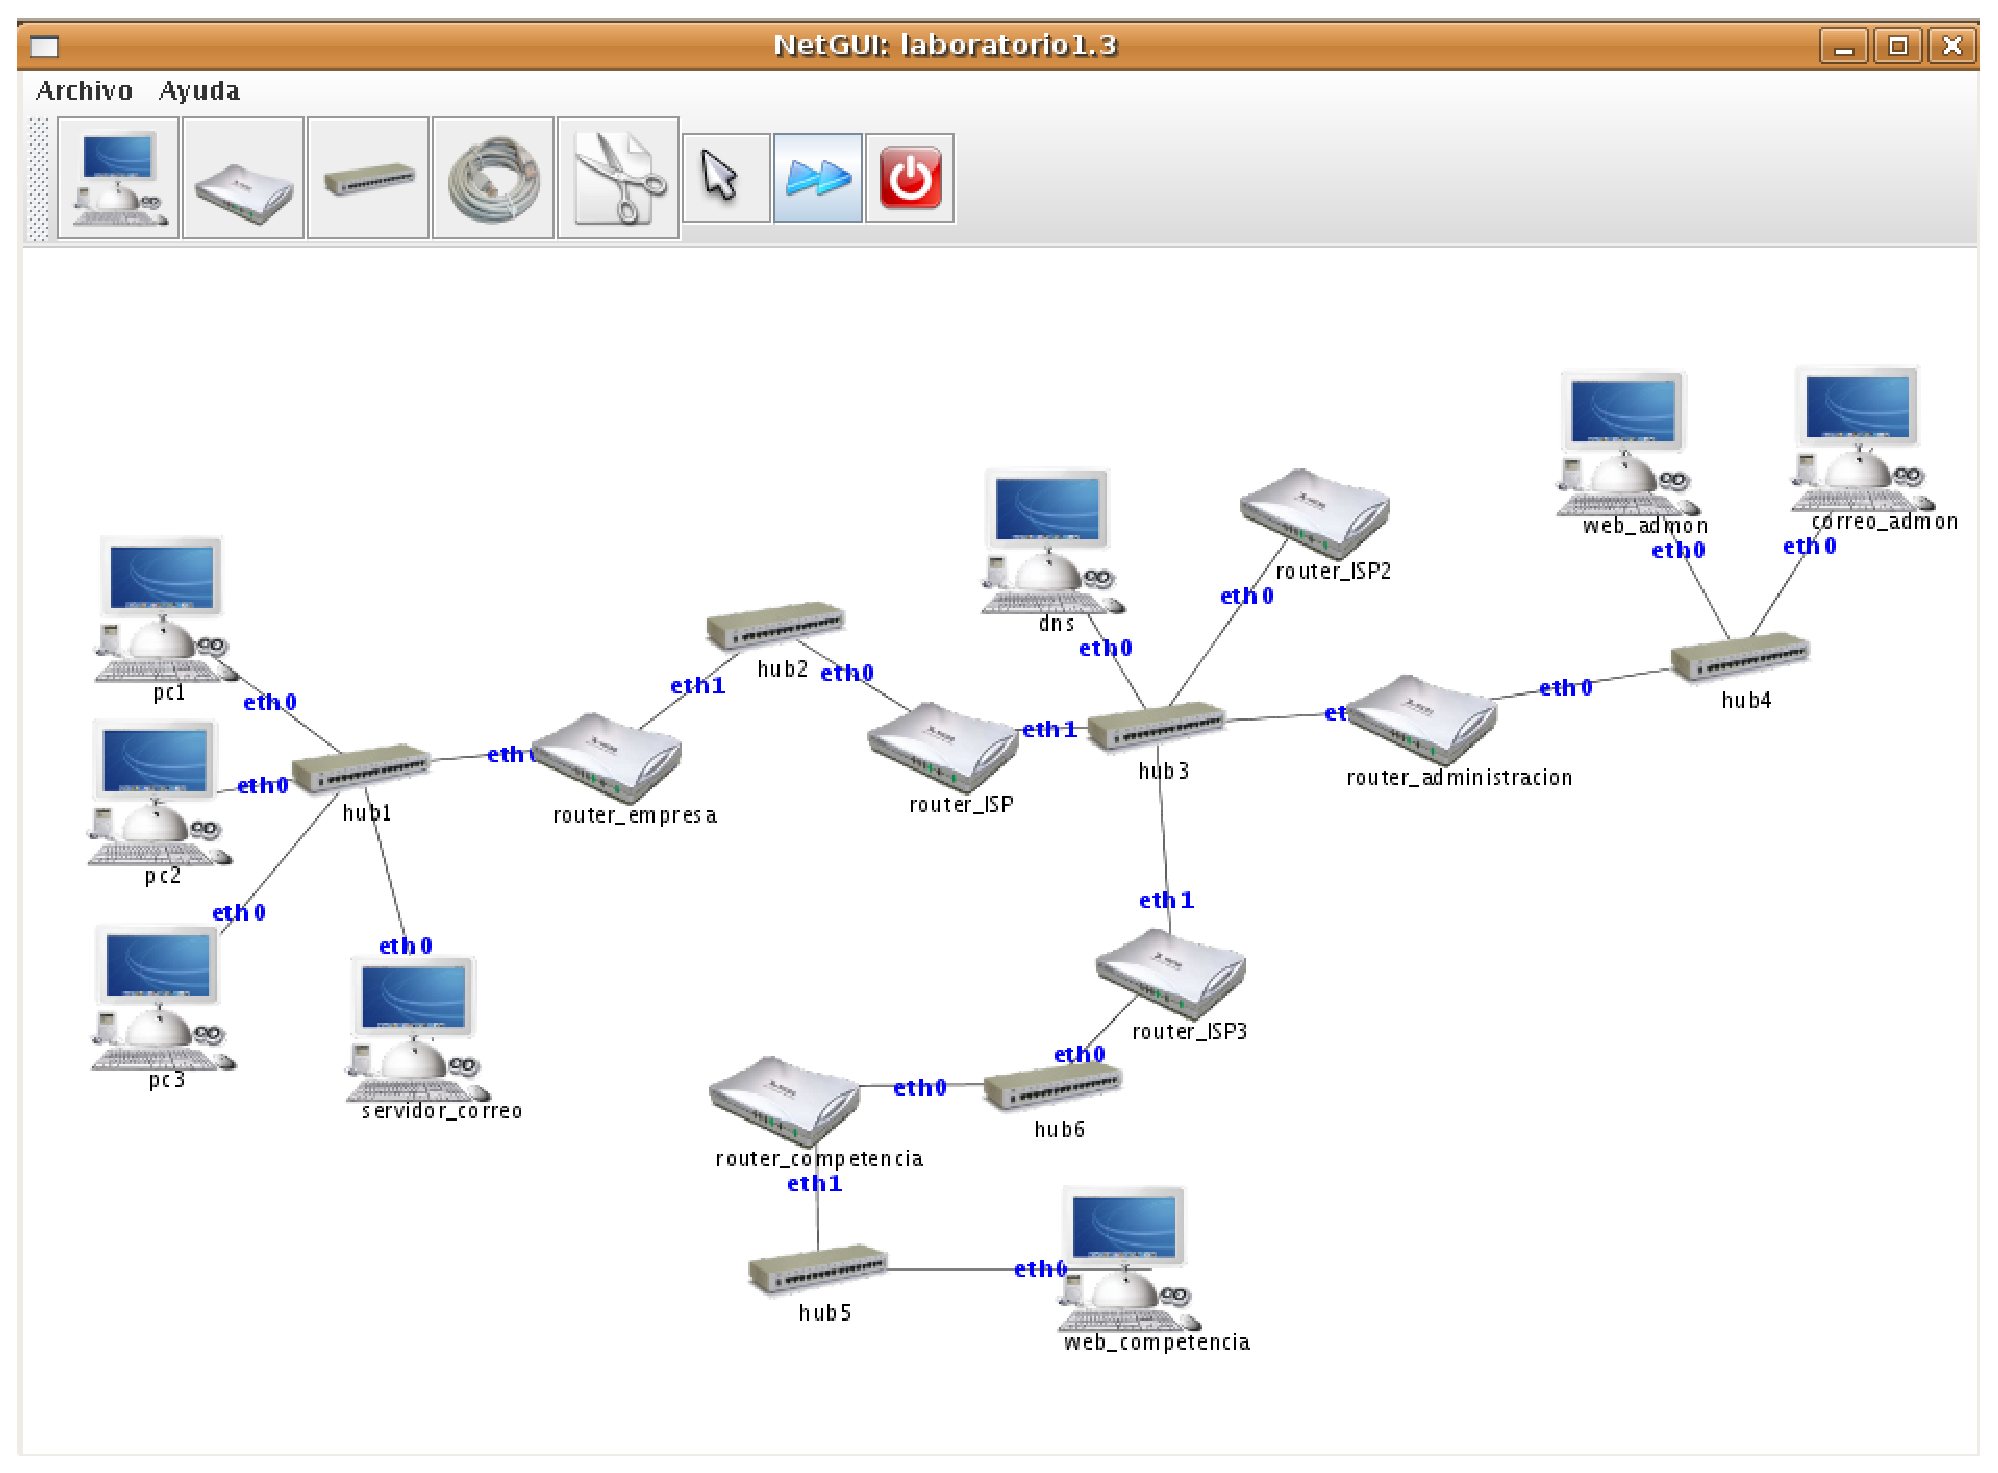
\includegraphics[width=6.9cm]{figs/netgui}}
\end{figure}
\end{minipage} \hfill
\
\begin{minipage}{4cm}
\begin{itemize} 
\item
\emph{Front-end} gráfico para Netkit
\item 
Desarrollado en GSyC
\end{itemize}
\end{minipage}\hfill
\end{frame}
%%---------------------------------------------------------------

%%---------------------------------------------------------------
\begin{frame}[fragile]

\frametitle{coLinux, AndLinux}

coLinux:
\begin{itemize}
\item
Año 2004. Basado en UML
\item
Actualmente en desuso
\item
Versión del núcleo de Linux que se ejecuta sobre otro S.O, como Windows
\end{itemize}

AndLinux
\begin{itemize}	
\item
Distribución basada en Ubuntu con
versión del núcleo de Linux para ejecutarse sobre Windows 2000, XP, 2003, Vista, 7 (solo las versiones de 32 bits)
\item
Usa coLinux
 
\item 
Algunos servicios van sobre Windows nativo: Servidor de X Window (Xming), servidor
de sonido (Pulse Audio)
\end{itemize}


\end{frame}







%%---------------------------------------------------------------
\section{Técnicas sin virtualización}
%%---------------------------------------------------------------
\begin{frame}[fragile]
\frametitle{Técnicas sin virtualización}
Instalación, reconfiguración y replicación automática, independecia de la plataforma,
portabilidad... son características deseables en una buena administración de sistemas


\begin{itemize}
\item
Todas ellas pueden conseguirse mediante virtualización

\item
Pero la virtualización no es la única forma. Hay multitud de técnicas de
administración alternativas que también ofrecen estas cualidades

\item
Un buen administrador de sistemas evaluará lo más adecuado para cada caso
\end{itemize}

Veremos a continuación alguna de estas técnicas


\end{frame}


%%---------------------------------------------------------------
\begin{frame}[fragile]
\frametitle{Jaulas chroot}
\begin{itemize}
\item
Se cambia el directorio raiz que percibe un proceso, (y sus hijos)
de forma que no puede acceder fuera de cierto directorio.
\item
No se aisla el acceso a otros procesos, memoria, CPU, red u otros dispositivos
\end{itemize}

\end{frame}



%%---------------------------------------------------------------
\begin{frame}[fragile]
\frametitle{Simuladores}
\begin{itemize}
\item
Simulan algunas características del comportamiento
externo de un sistema. P.e. simuladores de red
(\emph{GloMoSim}, \emph{JSIM}, \emph{ns-2}, \emph{OPNET}, \emph{OMNet}, etc)
\item
Los mal llamados
\emph{simulador de Zx-Spectrum para PC},
\emph{simulador de Commodore 64 para PC}, etc, no son simuladores. Son
emuladores completos.

\end{itemize}

\end{frame}


%%---------------------------------------------------------------

\begin{frame}[fragile]
\frametitle{Capas de Compatibilidad}

 \begin{itemize}
 \item
 Wine. Reimplementación de la API de Win16 y Win32 para sistemas 
 operativos basados en Unix bajo plataformas Intel. Permite
 ejecutar algunas aplicaciones para Windows en Linux. 

Cedega es un \emph{fork} comercial de Wine
 \item
 Cygwin. Año 1995.
 Entorno para portar software POSIX a Windows, compuesto por:
  \begin{enumerate}
  \item
  DLL que ofrece la funcionalidad de las llamadas al sistema de Linux
  \item
  Colección de herramientas habituales en sistemas Unix
  \end{enumerate}
  Siempre es necesario recompilar las aplicaciones 
\end{itemize}

\end{frame}
%%-----------------------------------------------------------

\begin{frame}[fragile]

\frametitle{Implementación de protocolos de red}

\begin{itemize}
\item
En redes Windows los directorios e impresoras se exportan mediante
los protocolos smb/cifs NetBIOS.

Samba es una implementación de estos protocolos,
permite
usar máquinas Unix en redes Windows 
\item
En Unix los directorios se exportan normalmente mediante NFS.
Hay implementaciones de NFS para Windows.  Permiten
acceder a directorios Unix desde máquinas Windows
\begin{itemize}
\item
En Unix las impresoras se exportan normalmente mediante LPD (\emph{Line Printer Daemon Protocol}).
Estándar basado en TCP, RFC 1179. 

Windows entiende este procolo, no hace falta software adicional
\end{itemize}
\end{itemize}
\end{frame}

%--------------------------------------------------------------------

\begin{frame}[fragile]
\frametitle{Clonación}
Permite replicar el disco de una máquina, y con ello todo su S.O. , configuración, aplicaciones y datos
\begin{itemize}
\item
Normalmente exige máquinas idénticas 
\item
Las herramientas suelen poder clonar cualquier máquina, con independencia de su S.O.
\begin{itemize}
\item Clonezilla. Libre, multiplataforma
\item Norton Ghost. Soft propietario para Windows
\item Acronis True Image.  Soft propietario para Windows
\item Partition Saving. Freeware para Windows
\item Partimage. Soft libre, basado en linux, permite clonar cualquier S.O.
Viene incluido en \emph{SystemRescueCd}, una distro \emph{live} orientada a 
recuperar y reparar un sistema
\item SystemImager. Soft libre para Linux. 

Uso típico:
  \begin{footnotesize}
Se instala un PC, el \emph{cliente de oro}. La imagen
se almacena en el servidor. Esta imagen de distribuye por la red (local), clonando
el PC. Si es necesario recuperar una imagen, solo se distribuyen los cambios
  \end{footnotesize}
\end{itemize}

\end{itemize}

\end{frame}

%%---------------------------------------------------------------
\begin{frame}[fragile]
\frametitle{Instalación automática del S.O.}
Sistema que contesta automáticamente a las preguntas que hace un SO en su instalación. 
\begin{itemize}
\item
\emph{preseed} (debian)
\item
\emph{kickstart (Red Hat)}
\item \emph{nLite} (Windows XP)
\item \emph{vLite} (Windows Vista)
\end{itemize}
\end{frame}

%%---------------------------------------------------------------
\begin{frame}[fragile]
\frametitle{Instalación automática de aplicaciones web}
Librerías de scripts que instalan aplicaciones web 
\begin{itemize}
\item
Muy usadas por los servicios de hosting

\item
El interfaz de usuario suele ser via web

\item
Las aplicaciones que soportan suelen ser aplicaciones para el web

\item
Ejemplos: Softaculous, Installatron, Fantastico

\end{itemize}

\end{frame}







%%---------------------------------------------------------------
\begin{frame}[fragile]
\frametitle{Herramientas de administración centralizada}
Herramientas que se encargan de que los ficheros
de configuración se \emph{mantengan} en cierto estado
(sin necesidad de preparar scripts que busquen las inconsistencias
y las corrijan)
\begin{itemize}
\item
cfengine

Herramienta tradicional, muy potente. Manejo de cierta complejidad
\item
landscape

Para ubuntu. De pago
\item
spacewalk

Para Red Hat y CentOS
\item
Puppet

Herramienta muy popular. Basada en Ruby. Algo pesada

\item
Ansible

Muy ligera, no necesita demonio en el cliente, solo ssh. En auge



\item
Chef, Bcfg2, otras alternativas
\end{itemize}

\end{frame}


\end{document}


